\section{Software}
\label{chptr:software}
% Beschreibe wie die Agile Softwareentwicklung in diesem Projekt verwendet wurde
Die Software wurde mit der plangesteuerten-agilen Softwareentwicklungsmethode realisiert. 
%Beschrieb was die Software machen soll und wie sie es machen soll und wie dies erreicht wurde, wie wurde die Software unterhalten und wie kam es überhaupt zur Programmiersprache Python?
Die Funktion der Software soll es sein, die Stabilisierung der Temperaturen der Pumpdiode und des Kristall zu gewährleisten. Daneben soll auch die Stromzufuhr für den Diodentreiber gesteuert werde können.\\
Die gesamte Programmierung der Steuerung wurde in der Programmiersprache Python erstellt. Die Rechner der Raspberry PI Serie sind dafür ausgelegt unter anderen hauptsächlich in den Sprachen Python als auch C/C++ programmiert zu werden. Es können Skripte erstellt werden, die direkten Zugriff auf Aus- und Eingänge haben und diese so steuern können. Im Rahmen dieser Arbeit wird nicht tiefer auf den Quellcode eingegangen, bei Interesse kann dieser im Anhang unter dem Abschnitt \ref{main_src} nachgelesen werden.\\
% Um die Versionierung der Softwarekomponenten aufrecht zu erhalten, wurde die Software \textit{Git} verwendet.

% \subsection{Softwarespezifikation}
% Analyse der Anforderungen, hier werden die verlangten Funktionen des Systems verstanden und Definiert. Für diese Software wurde eine inkrementeller Aufbau des Systems gewählt. So können im Nachhinein Anpassungen einfacher eingepflegt werden. $[6; S. 64-73]$

\subsection{Software Architektur}
\label{lab_software_architecture}
% Hinweise auf die Objektorientierung der Software.
In diesem Kapitel wird die Architektur der Software beschrieben. Auf Grund der Wiederverwendbarkeit und der Übersicht des Programms wurde die Software möglichst modular aufgebaut. Sämtliche Teile der Software wurden in funktionelle Komponente unterteilt. Es wird zwischen dem Backend und dem Frontend unterschieden, wobei beide wiederum in kleinere Komponente unterteilt werden. Ebenfalls zur Übersicht wurde das Programm in einige Unterprogramme aufgeteilt. So wird sowohl die Ausführung des GUI und die Auswertung der Daten der TECs, als auch die Steuerung des Diodentreibers und die Ansteuerung des TEC-Treibers in jeweils eigenen Unterprogrammen ausgewertet. Für die parallelen Abläufe im Programm wurde die Methode \textit{Threading} verwendet, auf das im Kapitel \ref{concurrency} \textit{Parallelität / Gleichzeitigkeit im Programm} eingegangen wurde. Daneben wurde die Programmstruktur nach dem \textit{Producer-Consumer}-Entwurfsmuster erstellt, was im nächsten Kapitel erläutert wird.

Zusätzlich musste die Sicherheit der bedienenden Person und der Komponenten des Laseraufbaus selber gewährleistet werden. Dazu mussten gewisse Sicherheitsvorkehrungen getroffen werden. Für das Einschalten der Diode, muss ein Schieber betätigt werden, ohne welchen die Freigabe zum Start des Diodentreibers nicht gegeben wird. Daneben muss verhindert werden, dass der der Diodentreiber zu viel Strom in den Laser einspeist. Die meisten dieser Vorkehrungen sind im Programmcodes untergebracht, andere mussten in der mitgelieferten Software der Komponenten konfiguriert werden, wie weiter oben im Kapitel \ref{label_tec_treiber} \textit{TEC-Treiber} erwähnt.
% Zusätzlich dürfen die TECs nicht mit zu viel Leistung betrieben werden, was zu deren Zerstörung führen könnte und dies auch die Diode in Mitleidenschaft ziehen könnte.

\begin{figure}[H]
    \centering
    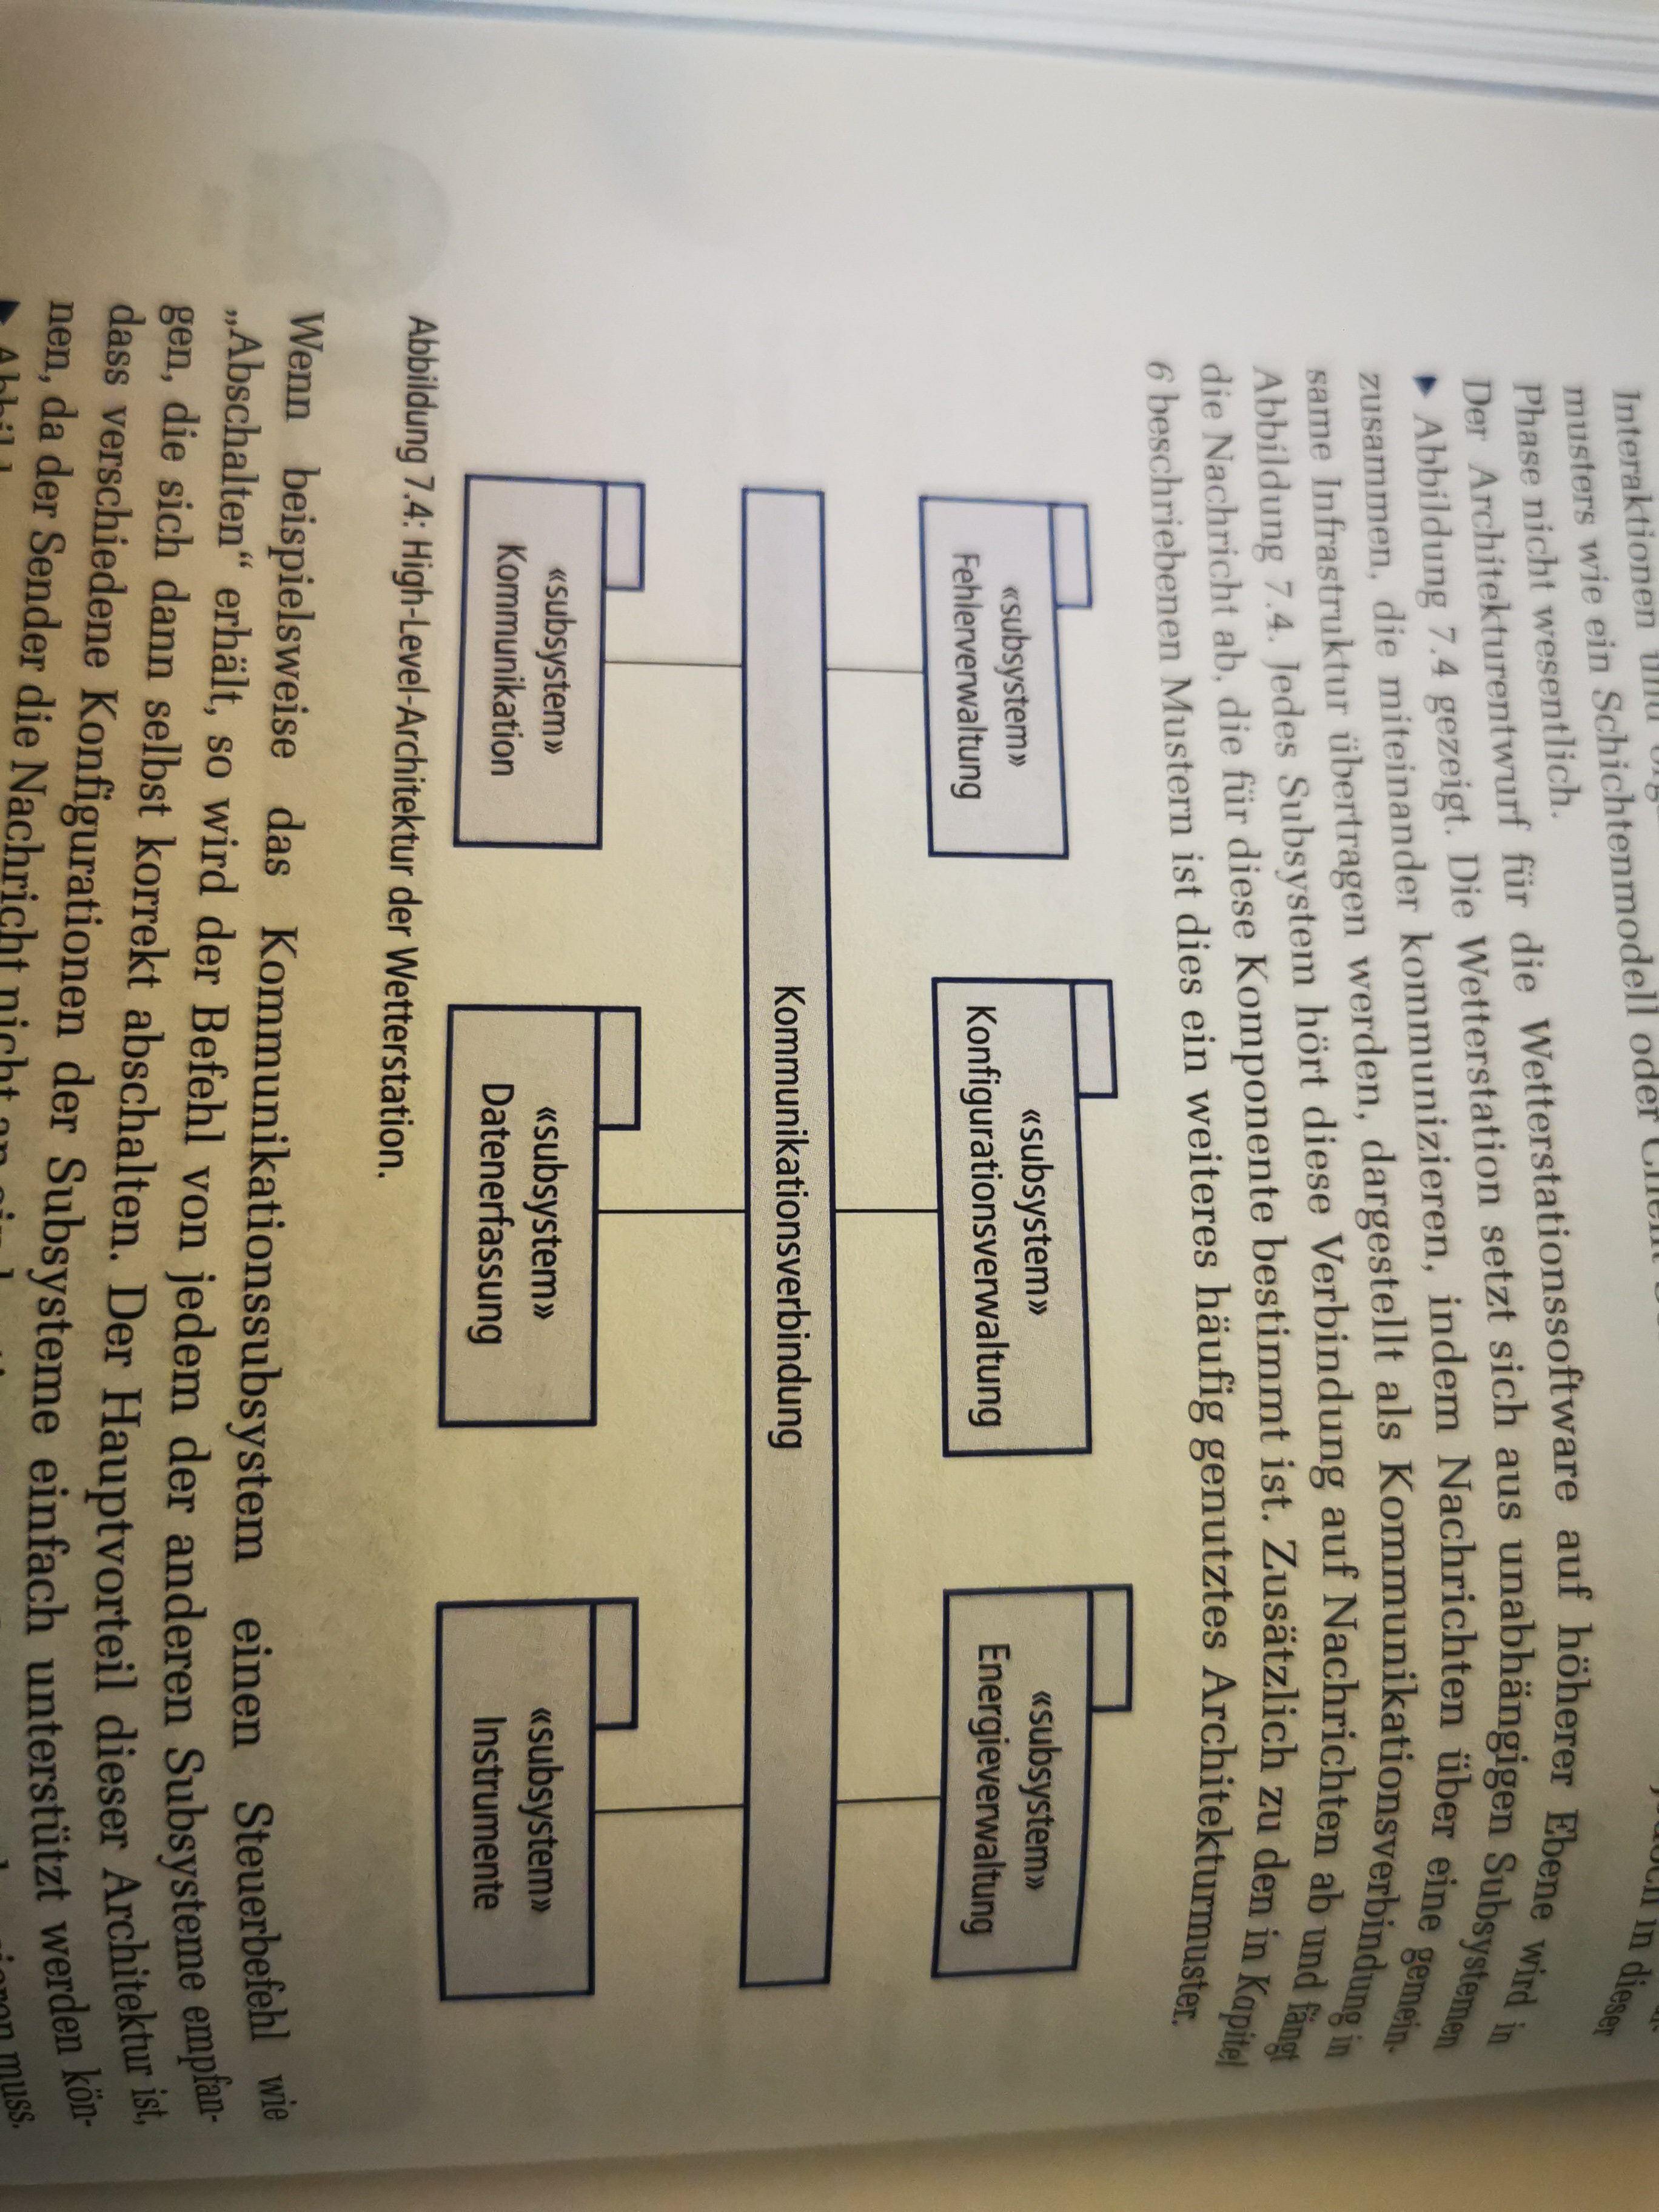
\includegraphics[scale=0.08, angle=90]{98_images/high_level_architecture.jpg}
    \caption{Die Architektur des Programms.}
    \label{fig:architecture}
\end{figure}

\subsubsection{Das Producer-Consumer Design-Pattern}
\label{section:_producer_consumer}
Die Bereitstellung der Daten der TECs und des Diodentreibers sind nach dem \textit{Producer} \textit{Consumer}-Design-Pattern aufgebaut. Das System besteht aus einem Teilnehmer, der Daten zur Verfügung stellt und einem oder mehreren Teilnehmer, die diese Daten beziehen. Die Daten werden vom \textit{Producer}, dem Datenproduzent in eine Liste, die sogenannte \textit{Queue} geschrieben, und von da vom \textit{Consumer}, dem Datenbezüger ausgelesen. Das Schreiben und Lesen der Daten in der \textit{Queue} folgt nach dem \textit{First-in First-out}-Prinzip, die Daten, die zuerst in die \textit{Queue} geschrieben werden, werden auch zuerst bezogen. Wird ein Datenpunkt aus der \textit{Queue} bezogen, wird dieser im selben Moment aus der \textit{Queue} gelöscht. Dies funktioniert stabil, auch wenn mit einem oder mehreren \textit{Threads} gearbeitet wird. $[7]$

Der Datentransfer der vorliegenden Steuerung musste zuverlässig sein. Aus diesem Grund wurde das \textit{Producer-Consumer}-Entwurfsmuster verwendet, auf welches im Abschnitt \ref{lab_software_architecture}  \textit{Softwarearchitektur} eingegangen wurde.

\begin{figure}[H]
    \centering
    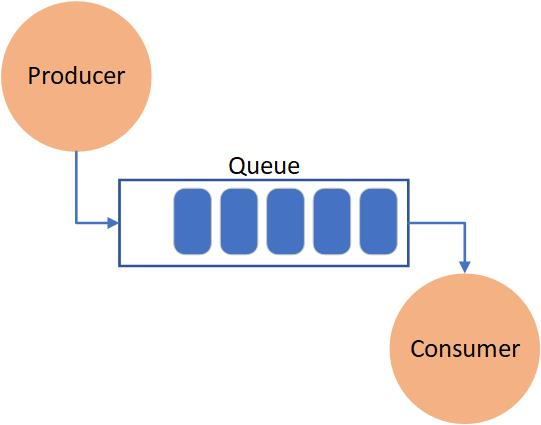
\includegraphics[scale=0.5]{98_images/producer_consumer_design_pattern.jpg}
    \caption{Das Prinzip des \textit{Producer-Consumer}-Entwurfsmusters.}
    \label{fig:_producer_consumer}
 \end{figure}

\subsection{Systemkontextmodell}
Das Systemkontextmodell beschreibt die anderen Systeme in der Umgebung und die Systemgrenzen. Der Aufbau des Kontrollers ist in Abb. \ref{fig:systemkontextmodell} ersichtlich. $[6]$

% \textbf{Architektur beschreiben.}

\begin{figure}[H]
    \centering
    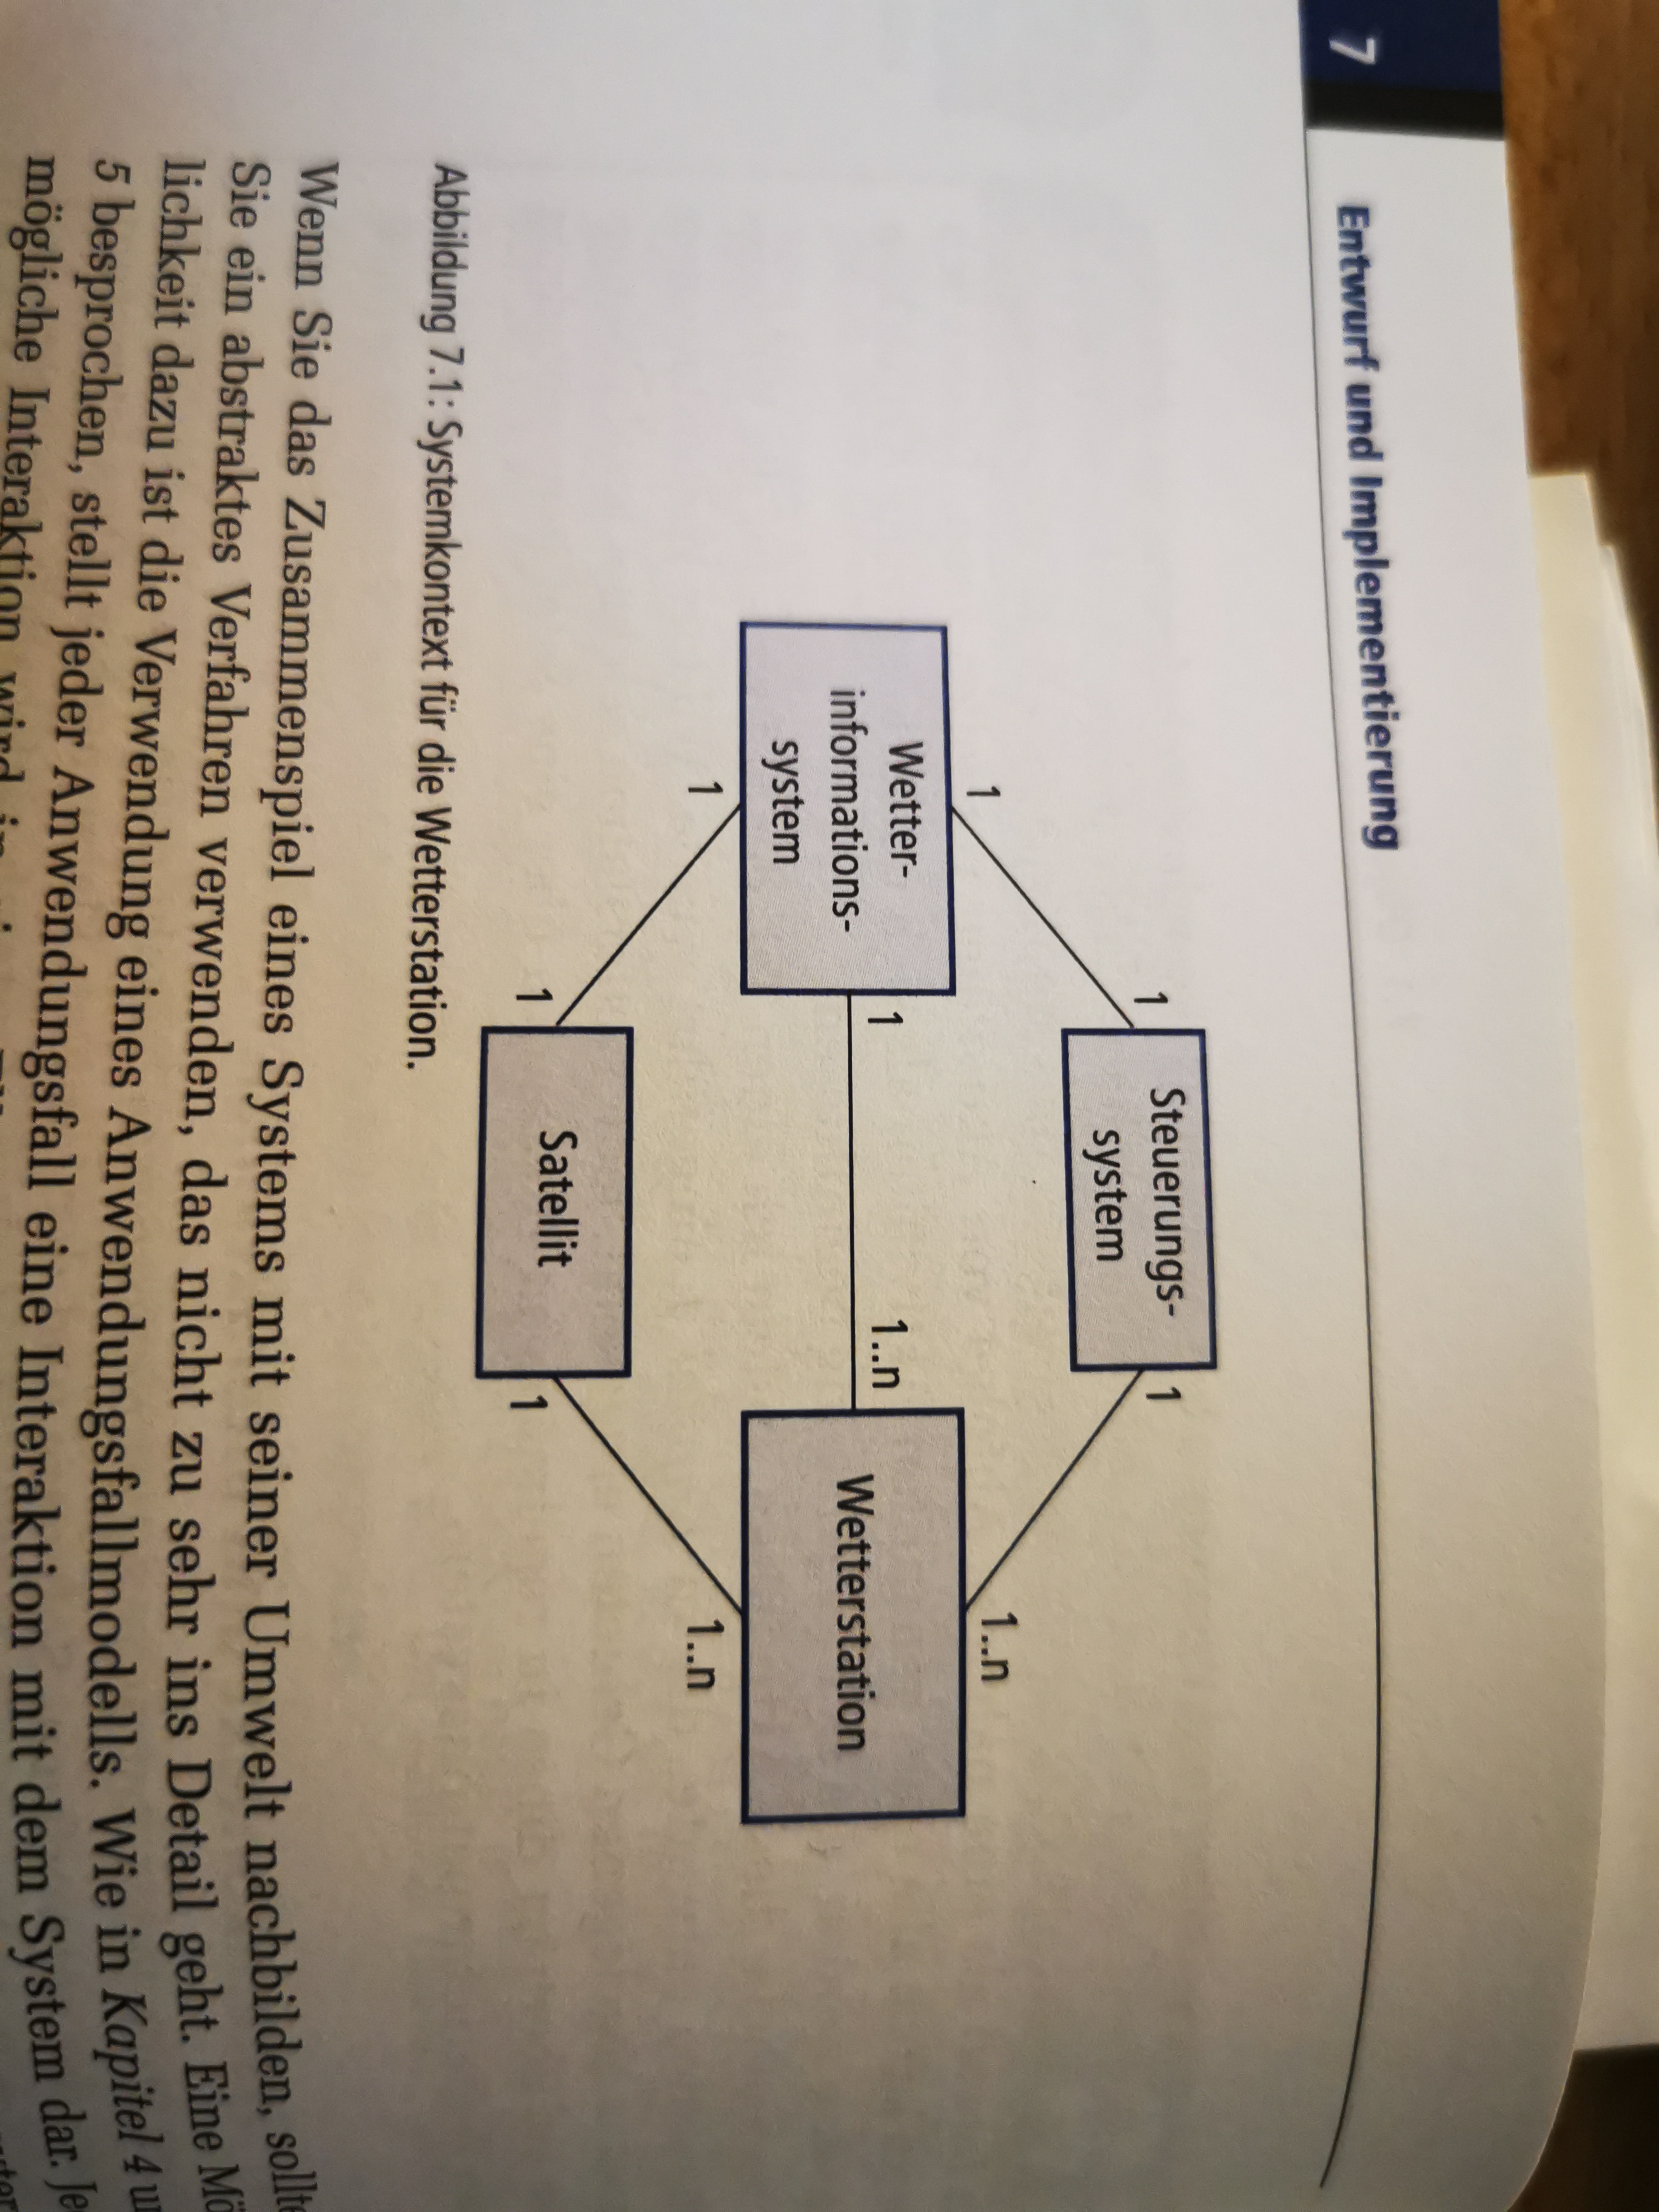
\includegraphics[scale=0.09, angle=90]{98_images/systemkontextmodell.jpg}
    \caption{Das Systemkontextmodell}
    \label{fig:systemkontextmodell}
\end{figure}

\subsection{Interaktionsmodell}
Das Interaktionsmodell zeigt auf, wie das System während der Benutzung mit seiner Umwelt zusammenspielt. Der Aufbau des Interaktionsmodells ist in Abb. \ref{fig:interaktionsmodell} gezeigt. $[6]$

\begin{figure}[H]
    \centering
    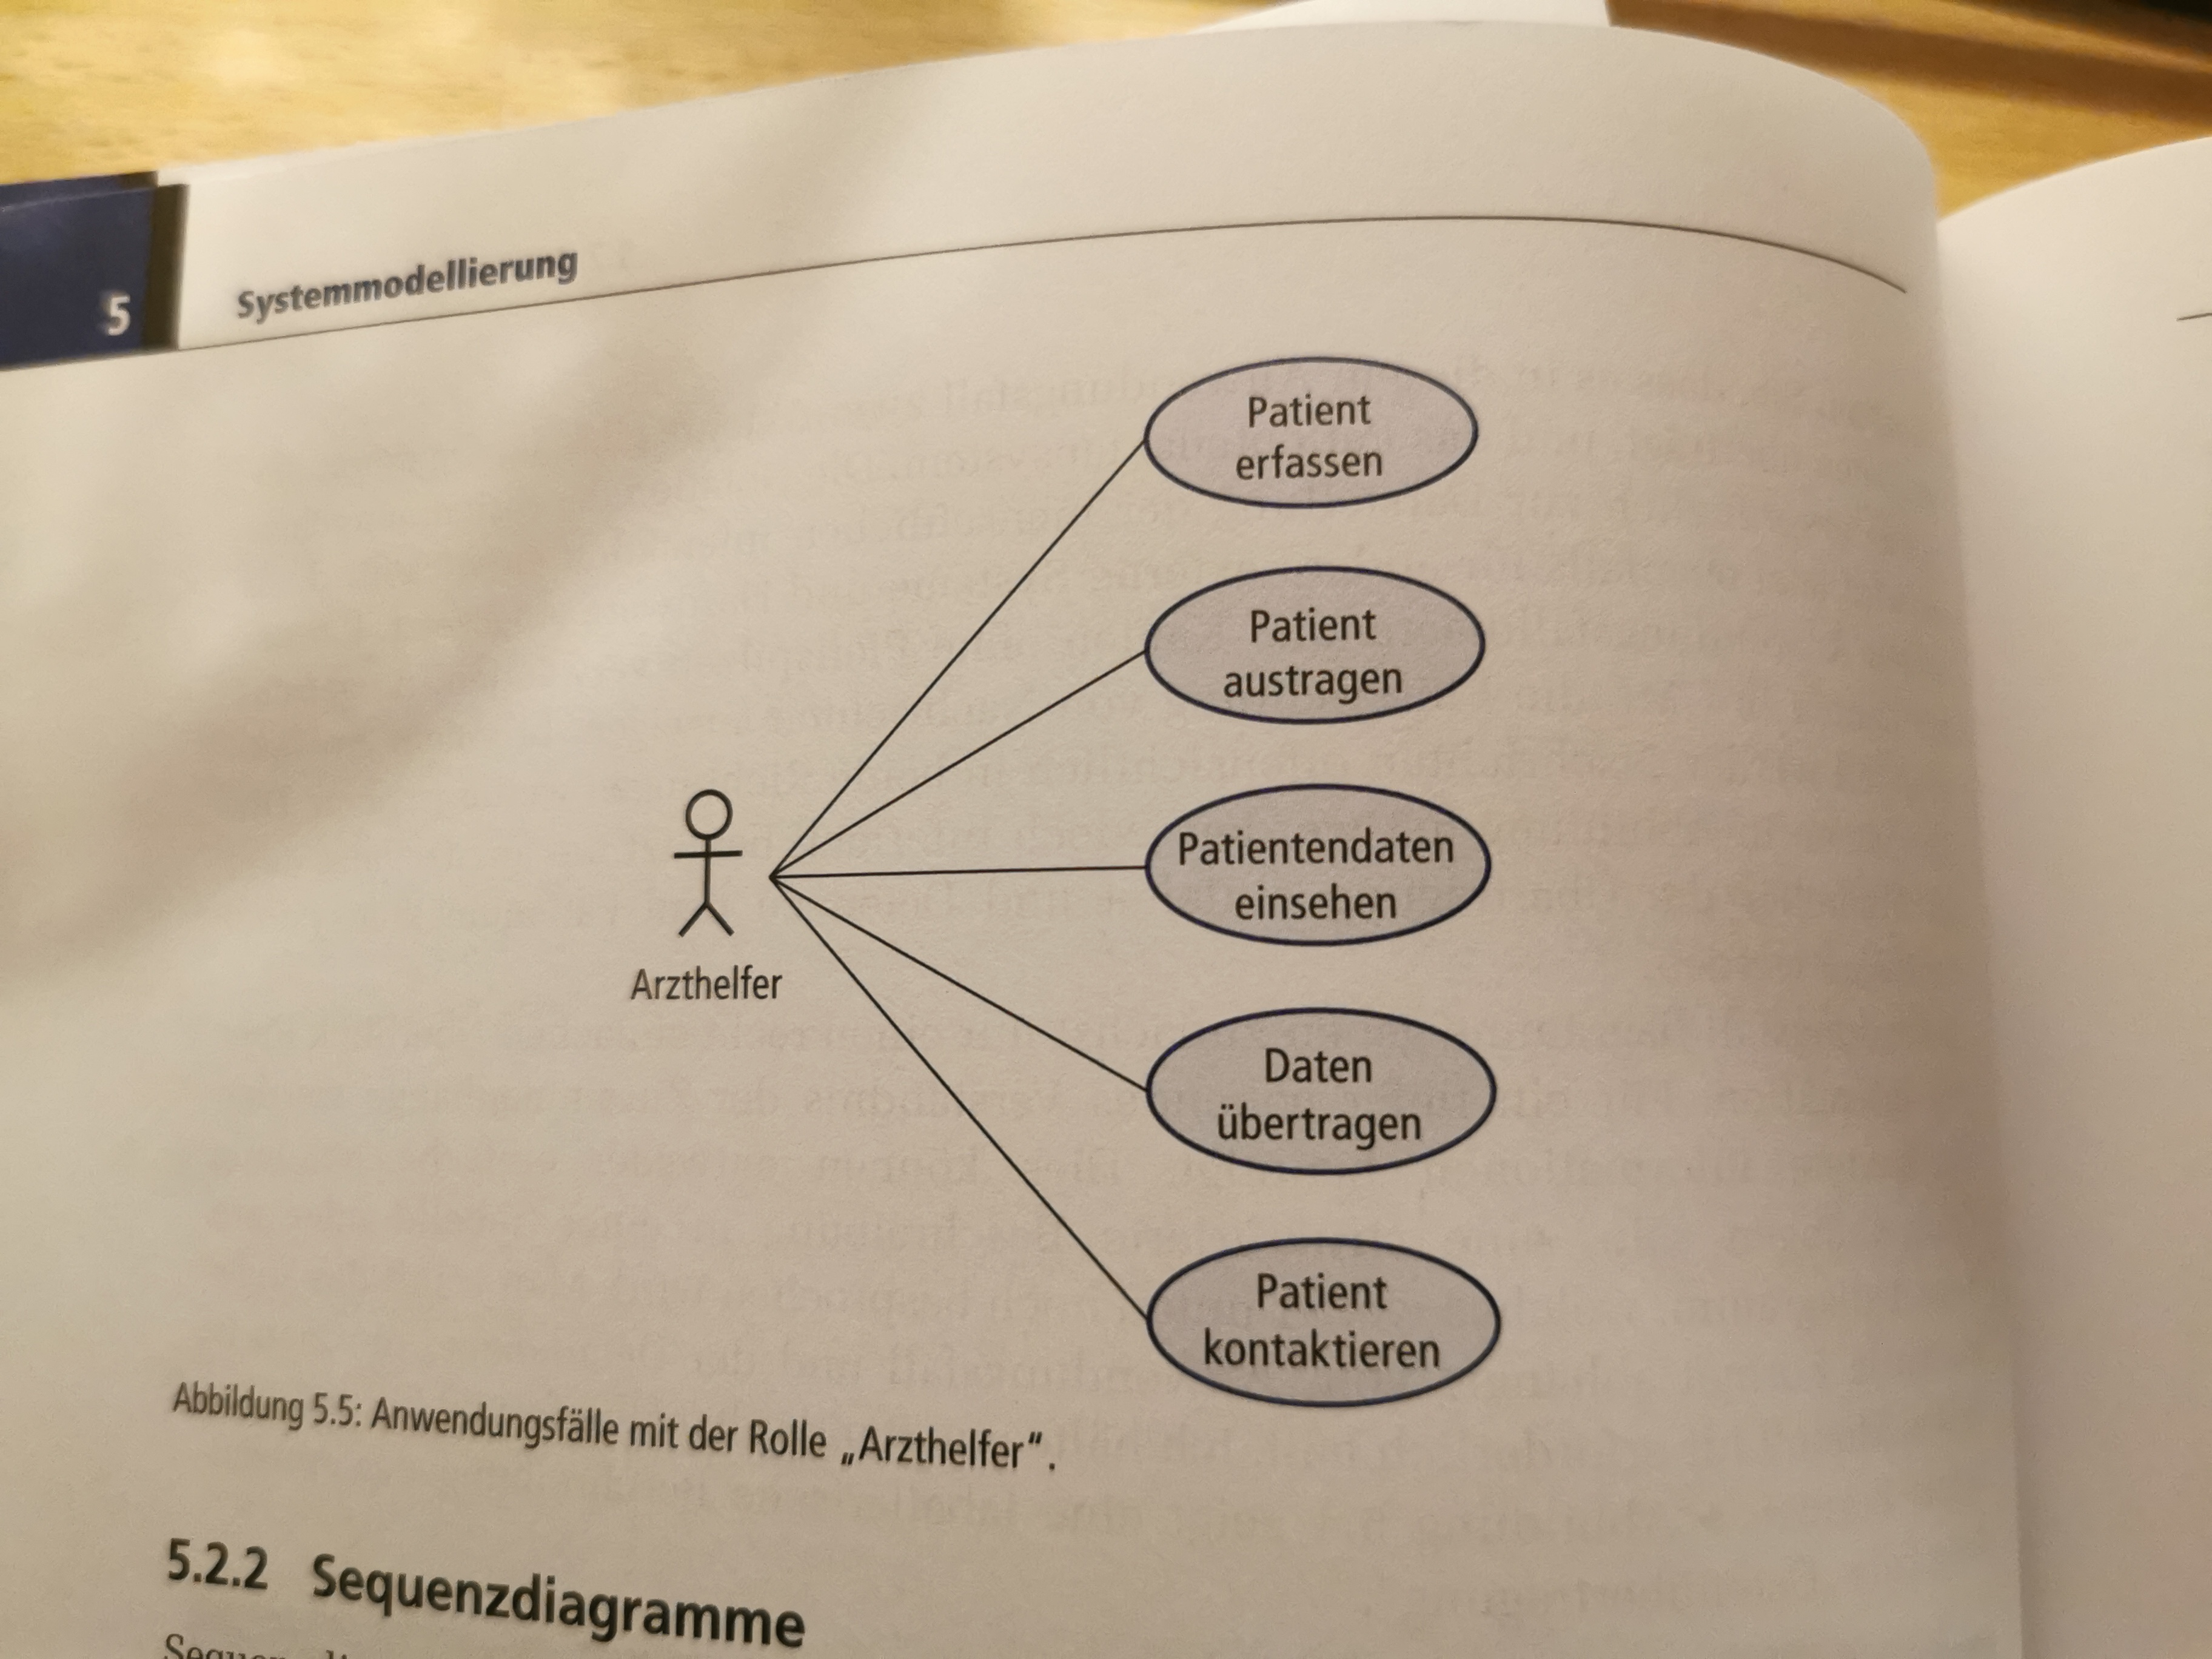
\includegraphics[scale=0.09]{98_images/interaktionsmodell.jpg}
    \caption{Das Interaktionsmodell}
    \label{fig:interaktionsmodell}
\end{figure}

\subsection{Datenorientierte Modellierung}
Die Datenorientierte Modellierung wurde verwendet, um den gesamten Datenfluss im Kontroller fest zu halten. Der Datenfluss im Kontroller ist in Abb. \ref{fig:dataflow_1} und in Abb. \ref{fig:dataflow_2} gezeigt. Der Datenfluss der Daten, die im Backend erzeugt werden, werden im Frontend dargestellt. Zu sehen ist die \textit{Queue}, in die die Daten zuerst geschrieben werden und erst von da von den Konsumenten bezogen werden. Eine Abzweigung geht in die Datenbank im Hintergrund. Aus Gründen der Handlichkeit, wurde das Datenformat .csv verwendet. Dies ist mit weitverbreiteten Drittanbietersoftware wie Excel von Microsoft kompatibel und kann mit einer Grösse von über einer Million Zeilen eingelesen werden. Zusätzlich ist beim einfachen öffnen der Datei die Zeichensetzung für Menschen lesbar. In der Abb. \ref{fig:dataflow_2} ist der Datenfluss der Daten, die im Frontend erzeugt werden und ins Backend transportiert werden dargestellt. Die Daten werden direkt und ohne in eine \textit{Queue} geschrieben zu werden ins Backend und dann an den TEC-Treiber und den Diodentreiber weiter gereicht. Das Weiterleiten der Daten an die Treiber im Backend wird vom Rechner an die angedachten Treiber weitergeleitet. Die beiden Datenströme sind getrennt dargestellt, einmal vom \textit{Backend} ins \textit{Frontend} und umgekehrt. $[6]$\\  % S.170
Die \textit{Queue} wurde deshalb eingesetzt, um eine bestimmte Datenstruktur zu gewährleisten. Dies ist möglich, weil die Daten gepuffert, also zwischengespeichert werden und nicht verloren gehen, sollte der Rechner einmal beschäftigt sein. Bei der Dateneingabe wird keine \textit{Queue} benötigt, die Eingabedaten sind nicht so dynamisch, wie die produzierten Daten, die Daten gehen nicht verloren.

Der \textit{Primary-Key} der .csv-Datei ist als Unix Zeitstempel dargestellt und wurde nicht in eine eine GMT-Zeit umgewandelt. Der Grund dafür ist, dass der Rechner keinen Internetzugang hat und die Zeit grundsätzlich nicht aktualisiert wird. Für die Darstellung der Werte spielt dies keine Rolle, weil die Werte relativ zur Zeit sind. Das Unix-Format jedoch ist in einer Tabelle einfacher zu handhaben, weil diese Werte nummerisch sind. Dazu müssen sie nicht mit Tabellenfunktionen konvertiert werden.\\

\begin{figure}[H]
    \centering
    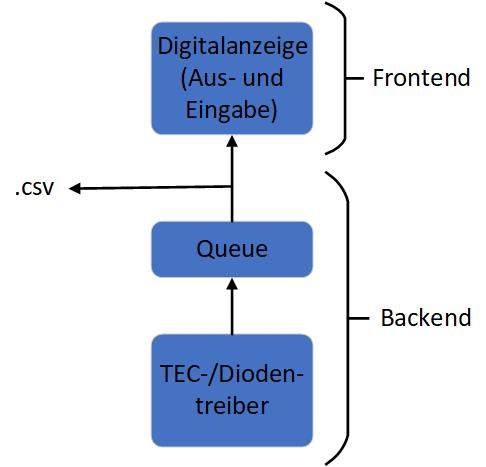
\includegraphics[scale=0.5]{98_images/data_oriented_back_front.jpg}
    \caption{Die datenorientierte Modellierung; Die Daten fliessen vom Backend zum Frontend.}
    \label{fig:dataflow_1}
\end{figure}

\begin{figure}[H]
    \centering
    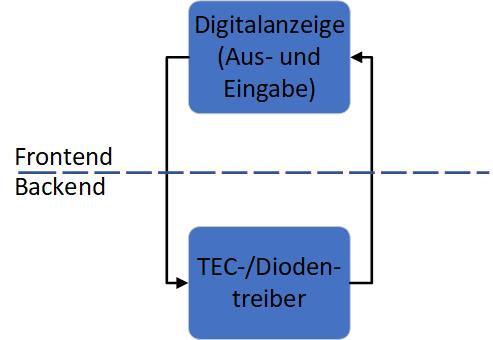
\includegraphics[scale=0.5]{98_images/data_oriented_front_back.jpg}
    \caption{Die datenorientierte Modellierung; Die Daten fliessen vom Frontend zum Backend.}
    \label{fig:dataflow_2}
\end{figure}

\subsubsection{Backend}
\label{chptr:software_backend}
Das \textit{Backend} umfasst in der Softwareentwicklung alle Programmiertätigkeiten, die die Logik in einer Software ausmachen. So werden Kommunikation zu Kontrollern aufgebaut, Daten in Datenbanken gespeichert und Daten ans Frontend gesendet und auch von da bezogen.

Die Objektorientierung wurde verwendet, wo dies möglich gewesen ist. Für die Erzeugung der Objekte wie Knöpfe, Rahmen oder Texten war dies nicht möglich auch wenn dies optimal gewesen wäre. Die Objekte wurden zwar erstellt, die Werte aktualisierten sich jedoch nicht. Die gesamte Anzeige ist somit in einer Initialisierungs-Funktion realisiert, die Funktion ist vollständig gegeben, dies entspricht jedoch nicht der gängigen guten Softwarepraxis. Die Übersicht bei einer Revision des Quellcodes ist somit erschwert. Ersichtlich ist dies im Quellcode im Anhang im Kapitel \ref{main_src}. Zeilen 23 bis 771 sind die Initial-Funktion

Die Ansteuerung des Diodentreibers wurde, wie weiter oben beschrieben mit einem analogen Signal realisiert. Dazu musste auf der SPS ein analoger Ausgang gesteuert werden.

Ansteuerung der TECs? - Über die API von Meerstetter wo bereits erwähnt?
Schemata sind in Abb. \ref{fig:dataflow_1} und \ref{fig:dataflow_2} gezeigt. Auf den Quellcode wird nicht eingegangen, bei Interesse kann dieser im Anhang unter dem Abschnitt \ref{main_src} nachgelesen werden.

\subsubsection{Frontend}
Das \textit{Frontend} umfasst alle Bereiche, die mit der Benutzeroberfläche (GUI) zu tun haben. So beinhaltet dies das Framework, mit dem das Design der GUI entwickelt worden ist und deren Benutzerführung. 
Die GUI soll alle benötigten und wichtigen Werte anzeigen und einzustellende Werte einlesen. Darunter sind die Anzeige der Temperaturen des Kristalls und der Pumpdiode im Bereich der Zieltemperaturen zu halten. Bei Notwendigkeit können die Solltemperaturen beider TECs geändert werden. Daneben besteht auch die Möglichkeit, den Nennstrom der Pumpdiode zu ändern. Neben den notwendigen angezeigten Werten, werden auch Werte zur Überwachung des Prozesses angezeigt. Um die Temperatur des Gehäuses zu überwachen, wird die Temperaturmessung des Prozessors des Raspberry PIs verwendet, mit der auf die Temperatur im Gehäuse der Steuerung geschlossen werden kann. Um den Anforderungen gerecht zu werden, wurden verschiedene Ansätze verfolgt die im Folgenden beschrieben werden. Dazu wurden teils Pro und Kontra vergleiche zur Hilfe gezogen.\\

Es war nicht möglich die Temperaturen als Graphen auf der Digitalanzeige darzustellen. Dies vor allem aus dem Grund, dass ich ergänzende Bibliotheken des Bibliothek \textit{Matplotlib} nicht in die Python-Umgebung einbinden konnte. Die Bibliothek \textit{Matplotlib}. Dazu konnte ich nicht garantieren, dass dies mit dem \textit{Threading / Multithreading} einwandfrei funktioniert.

\subsection{Evaluierung des Frameworks}
Für die Realisierung der Benutzeroberfläche musste das Framework evaluiert werden, mit der die Benutzeroberfläche erzeugt werden soll. Dafür werden die Frameworks \textit{Flask}, \textit{Tkinter} oder \textit{Customtkinter}, eine Erweiterung von \textit{Tkinter} der Programmiersprache Python benutzt/verwendet. Dazu standen die Optionen Webbasiert (in einem Webbrowser verwaltbar und nutzbar) oder eine Applikation zur Verfügung. Beide Optionen laufen lokal auf dem Rechner (Raspberry PI 3B+), dabei steht die Leistung des Rechners und die Handhabung der Oberfläche im Vordergrund. Die vom TEC-Kontroller ausgelesenen Werte, werden im Sekundentakt an den Rechner gesendet und müssen innerhalb dieser Sekunde ausgewertet werden können. Die Bedienung darf aus diesem Grund nicht zu viele Ressourcen des Rechners aufwenden. Dies konnte im Programm mit einer \textit{Queue} abgefangen werden. Dazu ist es wünschenswert, wenn die Benutzeroberfläche zur einfacheren Handhabung die gesamte Anzeige ausfüllt. Folgend werden die Dafür bzw. Dagegen sprechenden Argumente aufgelistet.
Neben dem oben genannten Framework wurden auch Bibliotheken von Drittanbietern, die nicht nativ in der Installation von Python vorhanden sind verwendet. Die Beschreibung derer sind in im Anhang unter dem Kapitel \ref{section:_libraries_py} gelistet und erläutert.

\begin{table}[H]
    \centering
    \begin{tabular}{l|l|l|l}
        \multicolumn{1}{c|}{$-$}&   \textbf{Webbasiert}&        \multicolumn{2}{c}{\textbf{Applikation}}\\
        \hline
        \textbf{Kriterium}&         \textbf{Flask}&             \textbf{Tkinter}&           \textbf{Customtkinter}\\
        \hline
        % Leistungseinbusse&        $=$ Mittel&                 $=$ Mittel&                 $=$ Mittel\\
        Schwierigkeitsgrad&         $-$ Mittel / Schwierig&     $+$ Mittel&                 $+$ Mittel\\
        Bibliothek&                 $-$ Standard&               $+$ Standard&               $+$ Standard\\
        Design&                     $+$ Vielfältig, schöner&    $-$ Weniger vielfältig&     $+$ Vielfältig\\
        Erfahrung&                  $-$ Keine Erfahrung&        $+$ Bereits Erfahrung&      $+$ Ähnlich Tkinter\\
        Programmiersprachen&        $-$ Python und HTML&        $+$ Python&                 $+$ Python\\
    \end{tabular}
    \caption{Evaluierung des Frameworks zur GUI Programmierung. Gelistet sind die Namen der jeweiligen Frameworks. \textit{Flask} ist das Framework der webbasierten Umgebung, wohingegen \textit{Tkinter} und \textit{Customtkinter} eigene Applikationen sind.}
    \label{tab:gui_programming}
\end{table}

Aus den Gründen der Erfahrung und der Anwendbarkeit mit Tkinter, fiel die Entscheidung auf die App-Variante. Zusätzlich konnte mit dem \textit{Customtkinter} Framework modernere Designs kreiert werden. Dies soll die Nutzung der Oberfläche vereinfachen. Es können somit ergonomische und ansprechende Designs realisiert werden.

\subsection{Die Anzeigen}
Die Anzeigen sehen wie in den folgenden Abb. \ref{fig:overview_sw} und \ref{fig:settings_sw} gezeigt aus. Die gesamte Anwendung wird im Vollbildschirm-Modus beim hochfahren des Rechners automatisch gestartet. Die englische Sprache für die Steuerung wurde aus dem Grund gewählt, weil damit die Nutzergruppe grösser ist.\\
Abb. \ref{fig:overview_sw} zeigt einen Überblick der Komponenten, der zugleich der Startbildschirm der Steuerung ist. Auf diesem werden alle wichtigen Parameter auf einen Blick angezeigt und können auch da eingestellt werden. Um die Benutzerführung zu vereinfachen, ist as Design ist in verschiedene Abschnitte unterteilt. So wurden Rahmen um die jeweiligen Steuereinheiten gelegt, damit klar ist wozu ein bestimmtes Element gehört. Zusätzlich ist die Anzeige in die Steuerung der TECs (auf der linken Hälfte) und die Pumpdiodentreiber (auf der rechten Hälfte) unterteilt, wobei die beiden TECs wiederum in den TEC des Kristalls und der Pumpdiode unterteilt wurde.\\
Angezeigt werden die aktuellen Werte, \textit{Acutal Value} der TECs, als auch der Strom des Diodentreibers. Bei allen dreien lassen sich die Sollwerte, \textit{Setpoint} der Temperaturen bzw. des Stromes mit den <<$+$>> und <<$-$>> Knöpfen hinter den Sollwerten erhöhen bzw. vermindern.
Der Schieberegler dient als Barriere zur Sicherheit, dass der Laser nicht bei unbeabsichtigtem Betätigen des Startknopfes den Laser startet. Bei Betätigen des \textit{Laser STOP}-Knopfes, kann der Laser zu jeder Zeit beendet werden.

Ersichtlich sind am oberen Rand zwei Schaltflächen, mit denen zwischen den zwei Anzeigen \textit{Overview} und \textit{Settings} gewechselt kann.

\begin{figure}[H]
    \centering
    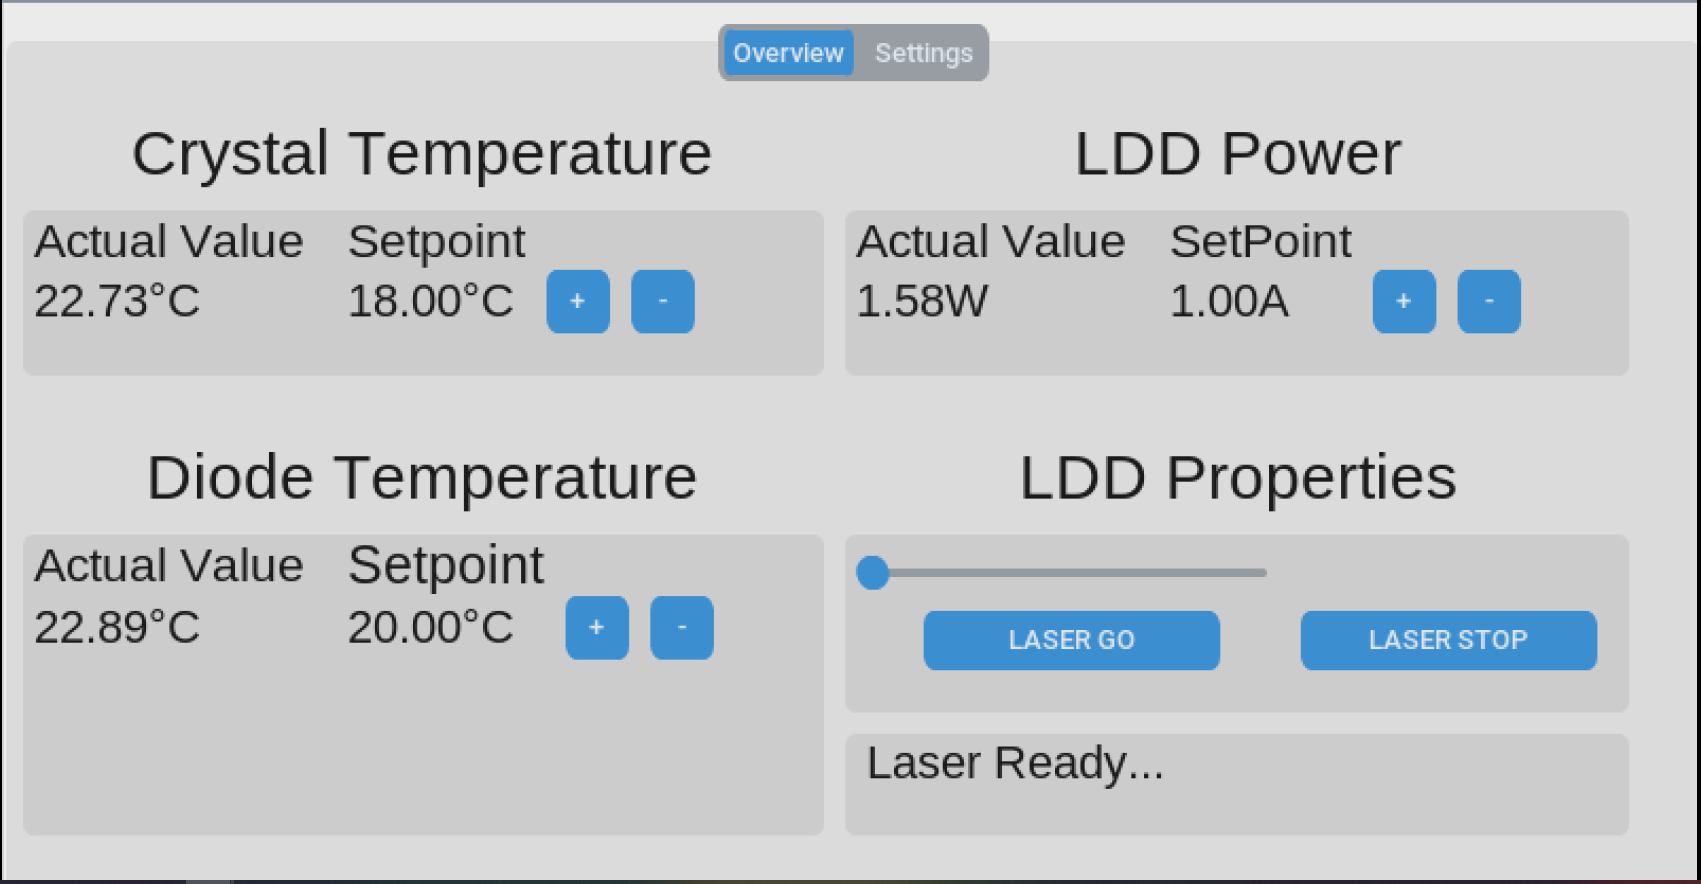
\includegraphics[scale=0.3, trim={1mm 1mm 1mm 1mm}, clip]{98_images/window_overview_large_04.PNG}
    \caption{Die Hauptseite \textit{Overview} der Steuerung}
    \label{fig:overview_sw}
\end{figure}

Gleich darunter befindet sich eine Statusanzeige für den Betrieb des Lasers. Folgende Texte werden je nach Status des Betriebes des Lasers angezeigt.

\begin{table}[H]
    \centering
    \begin{tabular}{l|l}
        \textbf{Text}&                          \textbf{Bedeutung}\\
        \hline
         \textit{Laser Ready}&                  Alle Bedingungen für den Start des Lasers sind erfüllt. Nun\\
         &                                      muss noch der Schieberegler betätigt werden und der Laser ist\\
         &                                      in Betrieb.\\
         \textit{Laser Running}&                Der Laser wurde gestartet und es wird ein Strom am Ausgang\\
         &                                      des Diodentreibers gemessen.\\
         \textit{Diode current above 1.5 A}&    Die Eingabe des Benutzers ist zu hoch, die 1.5A Limite des Di-\\
         &                                      odentreibers wurde überschritten.                                
    \end{tabular}
    \caption{Beschreibung der Texte für die Statusanzeige des Laserbetriebs.}
    \label{tab:my_label}
\end{table}

Abb. \ref{fig:settings_sw} zeigt verschiedene Parameter und Anwendungen. Um neben der Möglichkeit den Rechner herunter zu fahren und somit die Anwendung zu verlassen, können auch Daten exportiert oder das Design der Anzeige geändert werden.

\begin{figure}[H]
    \centering
    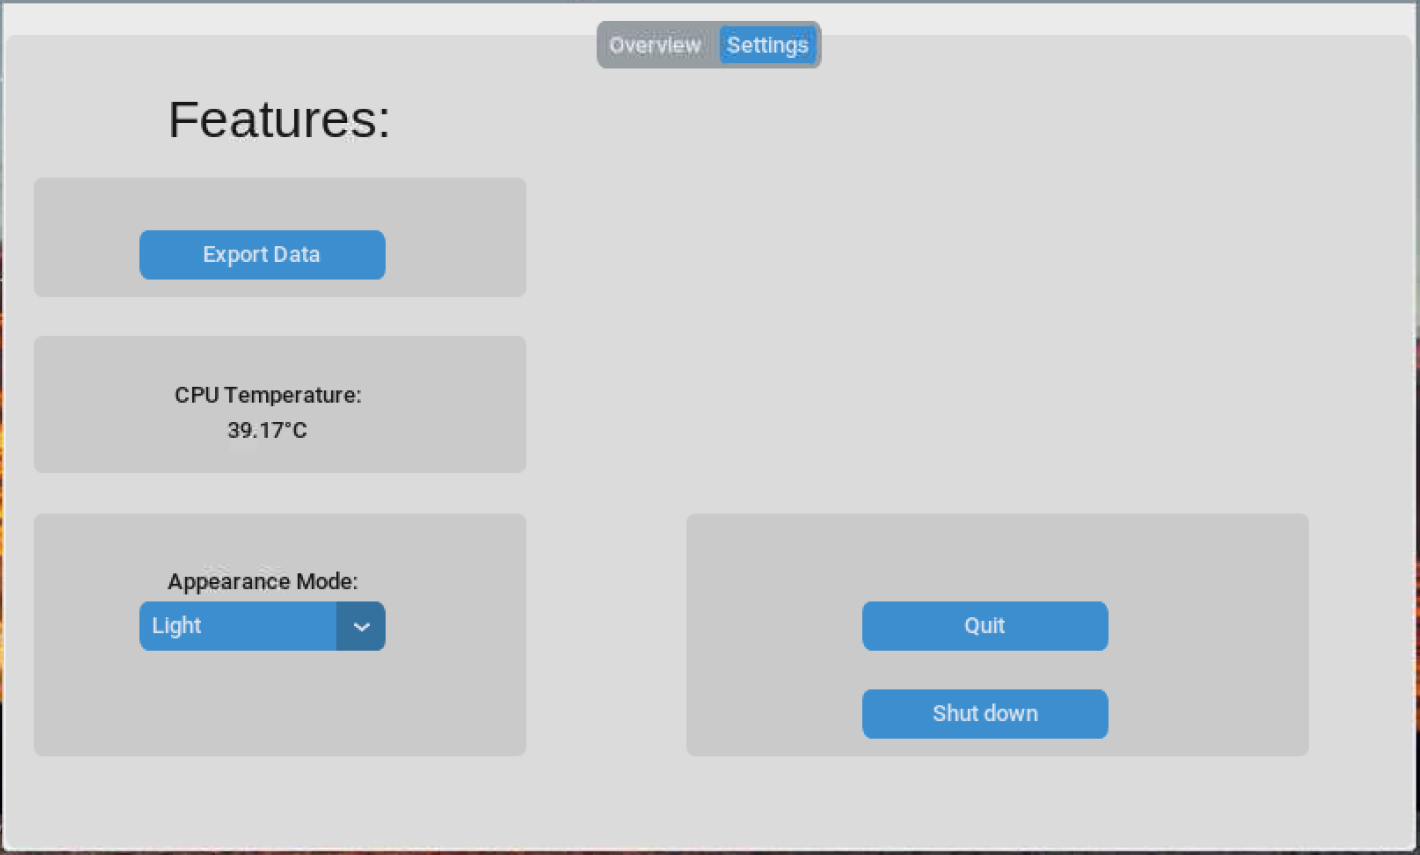
\includegraphics[scale=0.3, trim={1mm 1mm 1mm 2mm}, clip]{98_images/window_settings_large_02.PNG}
    \caption{Die Einstellungsseite \textit{Settings} der Steuerung}
    \label{fig:settings_sw}
\end{figure}

\begin{table}[H]
    \centering
    \begin{tabular}{l|l}
         \textbf{Anwendung}&        \textbf{Beschreibung}\\
         \hline
         \textit{Export Data}&      Exportiert die Temperaturen der TECs und die Ströme des Dioden-\\
         &                          treibers in einer .csv-Datei. Primary-key ist dabei die Zeit, alle Ein-\\
         &                          träge werden somit an Hand der Zeit sortiert.\\
         \textit{CPU Temperature}&  Anzeige für die Temperatur in der CPU des Rechners, diese sollte im\\
         &                          Bereich 40°C-65°C sein.\\
         \textit{Appearance Mode}&  Die gesamte Anzeige kann in einem hellen, als auch in einem dunkleren\\
         &                          Design erscheinen.\\
         \textit{Quit}&             Damit wird nur die Anwendung beendet und nicht der gesamten Rech-\\
         &                          ner heruntergefahren.\\
         \textit{Shut down}&        Bei Betätigung wird der gesamte Rechner herunter gefahren.
    \end{tabular}
    \caption{Beschreibung der Bedienung auf der \textit{Settings}-Anzeige}
    \label{tab:settings_beschriebung_sw}
\end{table}

\subsubsection{Kommunikation zwischen Backend - Frontend}

\begin{itemize}
    \item Mit welchen mitteln werden die Informationen aus dem Backend im Frontend angezeigt
    \item Kommunikation Raspberry PI - Digitalanzeige
    \item Kommunikation Raspberry PI - TECs
\end{itemize}

\textbf{Romain Caretto's Vorarbeit erwähnen}\\
\textbf{Neuster Stand der Technik}

\nocite{*}

% \subsection{Theorie 1}
% 
% \emph{Informieren und orientieren.} Das Schema in Abbildung~\ref{fig:software_struktur} enthält \ldots, \lipsum[7-7]
% 
% \lipsum[8]  Nach Formel \eqref{eq:sincos}:
% \begin{equation}
% \sin \alpha \pm \sin \beta = 2\sin\frac{\alpha\pm\beta}{2}\cos\frac{\alpha\mp\beta}{2}\,. \label{eq:sincos}
% \end{equation}

% \subsection{Softwareprototyp}
% \begin{enumerate}
%     \item Durchführbarkeitsstudie
%     \item Erhebung und Analyse der Anforderungen
%     \item Spezifikation der Anforderungen --> Als Liste realisieren(?)

%     \item Validierung der Anforderungen (Testen)
% \end{enumerate}
